\documentclass[a4paper,11pt]{article}
\usepackage[utf8]{inputenc}
\usepackage[spanish]{babel}
\usepackage[left=2.5cm,right=2.5cm,top=3cm,bottom=2.5cm]{geometry}
\usepackage{helvet} 
\renewcommand{\familydefault}{\sfdefault}
\usepackage{setspace}
\onehalfspacing 
\usepackage{graphicx}
\usepackage{float}
\usepackage{longtable}
\usepackage{booktabs}
\usepackage{tabularx}
\usepackage{hyperref}
\usepackage{enumitem}
\usepackage{caption}
\renewcommand{\LTcaptype}{figure}


% Configuración global de márgenes internos para todas las tablas
\setlength{\tabcolsep}{8pt}
\renewcommand{\arraystretch}{1.25}

\setcounter{secnumdepth}{5}
\setcounter{tocdepth}{5}

\setlength{\parindent}{0pt}

% Evitar la separación de palabras en sílabas y mantener justificado
\hyphenpenalty=10000
\exhyphenpenalty=10000
\sloppy

% Configurar \paragraph y \subsubsubsection con salto de línea (no en línea)
\makeatletter
    \renewcommand\paragraph{
        \@startsection{paragraph}{4}{\z@}%
            {-3.25ex\@plus -1ex \@minus -.2ex}%
            {1.5ex \@plus .2ex}%
            {\normalfont\normalsize\bfseries}
    }
    \newcommand{\subsubsubsection}{\paragraph}
\makeatother



\begin{document}

% --- PORTADA ---
\begin{titlepage}
    \centering
    \vspace*{1cm}
    {\large Universidad Nacional del Nordeste} \\
    {\large Facultad de Ciencias Exactas y Naturales y Agrimensura} \\
    \vspace{2cm}
    {\LARGE \textbf{Proyecto Integrador: Sistema de Administración de Consorcio}} \\
    \vspace{1cm}
    {\large Licenciatura en Sistemas de Información} \\
    \vspace{2cm}
    \vspace{2cm}
    \begin{flushleft}
        \textbf{Profesora:} Lic. Laura Gomez Solis \\
        \textbf{Integrantes:} \\
        \begin{itemize}
            \item Escobar, Lucas Joel
            \item Fernandez, Gabriel Elías
            \item Kern, Nicolás
            \item Solis Schneeberger, Matias
        \end{itemize}
    \end{flushleft}
    \vfill
    \vfill
    {\large Corrientes, 2026}
\end{titlepage}

%--- ÍNDICES ---
\tableofcontents
\newpage
\listoffigures
\newpage

%------------------ Introducción ------------------
\section{Introducción}

\subsection{Introducción}

La administración de consorcios de propiedad horizontal es una tarea compleja que requiere un manejo eficiente de recursos financieros, mantenimiento edilicio y mediación constante entre los residentes. Tradicionalmente, esta labor se ha sostenido mediante métodos manuales, uso de planillas de cálculo genéricas y comunicaciones en papel. El presente proyecto detalla el desarrollo de "CoConsorcio", un sistema web orientado a digitalizar, centralizar y optimizar la gestión integral de edificios, brindando herramientas automatizadas básicas tanto para el administrador como para los propietarios e inquilinos, buscando mejorar la transparencia y la convivencia de forma accesible.

\subsection{Breve estado del arte}

En la actualidad, la digitalización de la administración de propiedades ha cobrado impulso. Existen en el mercado plataformas comerciales de gran envergadura orientadas a corporaciones inmobiliarias. Sin embargo, estas herramientas de nivel empresarial suelen resultar económicamente inaccesibles para edificios pequeños o medianos, y presentan curvas de aprendizaje muy pronunciadas. En contraste, gran parte de las administraciones locales continúan operando de manera analógica, dependiendo de cuadernos físicos para el control de la guardia o de la distribución de expensas impresas. Esto evidencia una vacante para sistemas más ligeros, enfocados en resolver exclusivamente los problemas críticos diarios. CoConsorcio se posiciona en este segmento como una alternativa ágil, sirviendo como una prueba de concepto tecnológica ideal para aquellos consorcios que buscan dar su primer paso hacia la digitalización sin enfrentarse a sistemas sobredimensionados.

\subsection{Objetivos}

\textbf{Objetivo General:}  Desarrollar e implementar un sistema de información web (CoConsorcio) para la administración integral de consorcios, que optimice los procesos financieros, operativos y comunicacionales entre la administración, el personal de seguridad y los residentes.

\textbf{Objetivos Específicos:}
\begin{itemize}
    \item Automatizar el cálculo y prorrateo de liquidaciones mensuales de expensas, reduciendo el margen de error del cálculo manual.
    \item Implementar una integración inicial con pasarelas de pago (MercadoPago) que permita a los residentes abonar sus deudas de forma electrónica.
    \item Digitalizar la gestión de espacios comunes mediante un calendario interactivo para evitar conflictos y superposiciones de reservas.
    \item Centralizar la comunicación institucional mediante un muro de anuncios y un repositorio para la documentación del consorcio.
    \item Proveer una interfaz de control básica para el personal de seguridad, orientada al registro de visitas y paquetería.
\end{itemize}

\subsection{Fundamentación}

El desarrollo de este software surge como respuesta a las problemáticas detectadas en la gestión cotidiana de los edificios, representando a su vez una oportunidad invaluable para aplicar y consolidar los principios de la ingeniería de software en un entorno real. La dependencia de procesos manuales genera demoras en la recaudación y falta de transparencia. Se vuelve imperativo proponer soluciones tecnológicas que reemplacen prácticas obsoletas, como los cuadernos físicos de guardia, que son vulnerables a pérdidas y alteraciones. CoConsorcio se justifica técnica y académicamente al plantear una herramienta acotada pero robusta, construida bajo estándares modernos de desarrollo web, que moderniza el flujo de trabajo del administrador y empodera al vecino. Al tratarse de un proyecto gestado en el ámbito universitario, su diseño prioriza el código limpio, la escalabilidad y la correcta aplicación de metodologías ágiles por sobre la saturación de funcionalidades.


%--------------------------------------------------
\newpage

%------------------ Metodología ------------------
\section{Metodología}

\subsection{Ciclo de Vida - Metodología - SCRUM}

Scrum es una metodología ágil. Contiene un marco de trabajo adaptable, iterativo, rápido, flexible y eficaz, diseñado para ofrecer un valor considerable de forma rápida a lo largo del proyecto. Para cada proyecto que se aplique esta metodología se debe utilizar los principios scrum que son sus lineamientos básicos para la aplicación de su marco de trabajo y sus aspectos. A continuación, se mencionan las características de los principios y los aspectos del mismo.

\textbf{Principios de Scrum}
\begin{enumerate}
    \item Control del proceso empírico (Empirical Process Control)
    \item Autoorganización (Self-organization)
    \item Colaboración (Collaboration)
    \item Priorización basada en valor (Value-based Prioritization)
    \item Time-boxing
    \item Desarrollo iterativo (Iterative Development)
\end{enumerate}

\textbf{Aspectos de Scrum}
\begin{enumerate}
    \item \textbf{Organización}: Entiende los roles y responsabilidades definidos del proyecto con fines de asegurar la implementación exitosa de Scrum. Los roles de Scrum se dividen en 2 categorías: roles centrales (\textbf{Product Owner}, \textbf{Scrum Master}, \textbf{Equipo Scrum}) y roles no centrales (Interesados del negocio, clientes, usuarios y patrocinadores/sponsors).  
    \item \textbf{Justificación del negocio}: Se lleva a cabo una evaluación adecuada del negocio antes de iniciar el proyecto.  
    \item \textbf{Calidad}: Es la capacidad con la que cuenta el producto o los entregables para cumplir los con los criterios de aceptación y de alcanzar el valor de negocio esperado por el cliente.  
    \item \textbf{Cambio}: Los miembros del equipo del proyecto deben entender que los procesos de desarrollo están diseñados para el cambio.  
    \item \textbf{Riesgo}: Son una serie de eventos inciertos que pueden afectar los objetivos de un proyecto y pueden contribuir a su éxito o fracaso. Los riesgos que puedan tener impacto positivo en el proyecto, son considerados como oportunidades, mientras los riesgos que puedan tener impacto negativo en el proyecto se les conoce como amenazas.
\end{enumerate}

\subsubsection{Fase - Inicio}

\textbf{Visión del proyecto.}

Para administradores, vecinos y propietarios del edificio que necesiten resolver la desorganización y demoras en las gestiones diarias, nuestro \textbf{Sistema de Administración de consorcio} es una plataforma digital centralizada que automatiza liquidación de expensas, facilita la gestión de vecinos, implementa seguridad tanto dentro del edificio como fuera del mismo y agiliza la comunicación entre Inquilinos/propietarios del edificio. A diferencia de métodos manuales como Whatsapp o papel, en \textbf{nuestro sistema se garantiza una transparencia, comunicación rápida and efectiva con un control eficiente} de los recursos del edificio. Hemos identificado a \textbf{Fernández Gabriel Elías} como \textbf{Product Owner} por la visión del proyecto que proporcionó.

\textbf{Identificación del Scrum Master.}

Bajo los criterios de: \textbf{buen liderazgo}, \textbf{asignación de trabajo para los miembros dependiendo de sus habilidades en programación} y \textbf{actitud ante las adversidades}, identificamos a \textbf{Matías Solis Schneeberger} como nuestro \textbf{Scrum Master}, que nos guiará en este proyecto.

\textbf{Formación Equipo Scrum.}

Nuestro \textbf{Product Owner} con la colaboración del \textbf{Scrum Master}, ha seleccionado a \textbf{Escobar Lucas Joel} y \textbf{Nicolás Kern}, como miembros del equipo Scrum.

\textbf{Desarrollo de épicas y creación del backlog priorizado del Producto.}

Con la declaración de la visión del proyecto hemos podido lograr \textbf{desarrollar las épicas esenciales} para nuestro sistema. A continuación se muestran las épicas desarrolladas junto al \textbf{Backlog priorizando el producto.}

\begin{figure}[H]
    \centering
    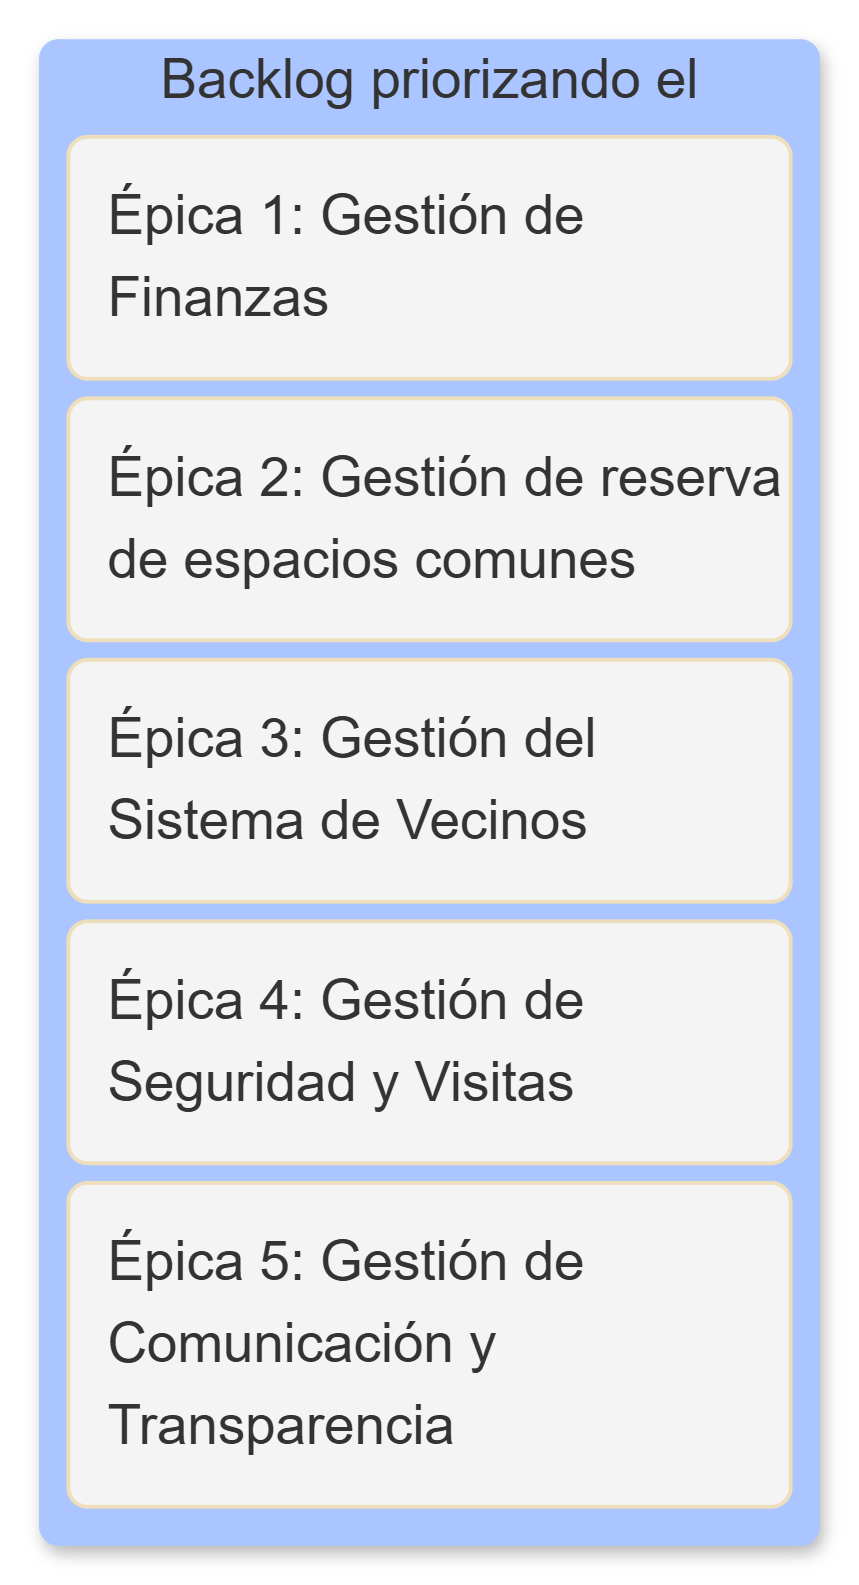
\includegraphics[width=0.313\textwidth]{figures/lista-de-backlog-con-las-epicas.png}
    \caption{Lista de BackLog con las épicas.}
\end{figure}



\textbf{Planificación de la liberación}

Tras el análisis del \textit{Product Backlog}, el Equipo Scrum ha priorizado las entregas basándose en el valor de negocio. Se determinó que el núcleo del sistema es el módulo contable, por lo que la Épica 1 (Gestión de Finanzas) conformará la primera liberación. Las entregas subsecuentes abordarán la gestión de reservas, usuarios, seguridad y comunicación.  

\textbf{Liberación 1: Gestión Financiera Base (Duración: 2 Sprints de 2 semanas)}
Para esta primera entrega, aplicamos una estricta priorización, seleccionando únicamente las Historias de Usuario (HU) críticas para el funcionamiento empírico del sistema, divididas en tres ejes:
\begin{itemize}
    \item \textbf{Estructura Base:} HU1 (Registro del Edificio) y HU2 (Configuración de Departamentos/ Alquileres). Son dependencias absolutas; sin la configuración inicial, el sistema carece de viabilidad.
    \item \textbf{Motor de Expensas (Administrador):} HU3 (Ingreso de Gastos), HU5 (Generar liquidación mensual) y HU6 (Registro manual de pagos). Permiten el registro de facturas, la generación de totales y el control de transferencias.  
    \item \textbf{Visibilidad (Inquilino/Propietario):} HU11 (Consultar mi estado de deudas), HU15 (Consultar gastos de expensa mensual) y HU13 (Pagar de deudas Online). Garantizan que el usuario final tenga claridad inmediata sobre su estado de cuenta.
\end{itemize}

Las funcionalidades secundarias de la Épica 1 (HU7 - Cálculo automático de intereses, HU10 - Notificaciones automáticas, HU14 - Subir comprobante y HU16 - Confirmar pago por transferencia) permanecerán en el \textit{Product Backlog} para iteraciones futuras, mitigando así los riesgos técnicos de esta primera entrega.  

\textbf{Liberación 2: Gestión de Espacios y Usuarios (Duración: 2 Sprints de 2 semanas)}
Esta liberación integrará las funcionalidades esenciales de dos grandes módulos para expandir el valor entregado al consorcio:
\begin{itemize}
    \item \textbf{Épica 2 (Reserva de espacios comunes):} Se implementarán la HU17 (Ver disponibilidad), HU18 (Solicitar reserva) y HU20 (Cancelar reserva), dejando el módulo operativo para los residentes.  
    \item \textbf{Épica 3 (Sistema de Inquilinos/Propietarios):} Se abordarán la HU22 (Alta de usuario), HU23 (Actualización de datos) y HU24 (Baja o desvinculación). Las tareas de gestión administrativa profunda (HU19, HU21 y HU25) se postergan para evitar comprometer los plazos y la estabilidad del incremento.
\end{itemize}

\textbf{Liberación 3: Seguridad y Transparencia (Duración: 2 Sprints de 2 semanas)}
Dado que la complejidad técnica y el esfuerzo estimado de las épicas restantes es menor, esta entrega abarca la totalidad de las funcionalidades planificadas para los módulos 4 y 5, sin representar un riesgo para el cronograma del proyecto:
\begin{itemize}
    \item \textbf{Épica 4 (Seguridad y Visitas):} HU26 (Ingreso de visita), HU27 (Recepción de paquetería) y HU28 (Confirmar retiro).  
    \item \textbf{Épica 5 (Comunicación):} HU29 (Publicar comunicado), HU30 (Consultar documentos) y HU31 (Enviar consulta a administración).
\end{itemize}

\subsubsection{Fase - Planificación y Estimación}

\paragraph{Creación de historias de Usuario.}
Durante la fase de Planificación y Estimación, el equipo procedió a desglosar las Épicas en requerimientos granulares. Se utilizó el formato estándar de roles y la técnica de comportamiento (Dado/Cuando/Entonces) para los criterios de aceptación, asegurando que cada funcionalidad aporte valor al consorcio. A continuación historias críticas detalladas a modo de ejemplo.

\begin{figure}[H]
    \centering
    \begin{tabular}{|p{\dimexpr\textwidth-2\tabcolsep-2\arrayrulewidth\relax}|}
        \hline
            \multicolumn{1}{|c|}{\textbf{Historia de Usuario 1: Registro del Edificio}} 
        \\ \hline

            \textbf{Descripción:} 
            \begin{list}{}{} 
                \item \textbf{Como} administrador 
                \item \textbf{Quiero} registrar un nuevo edificio en el sistema definiendo su información general y el desglose de unidades funcionales 
                \item \textbf{Para} crear el marco estructural necesario sobre el cual se basará toda la gestión administrativa. 
            \end{list}
        \\ \hline
        
            \textbf{Criterios de Aceptación:} 
            
            \begin{list}{\textbullet}{} 
                \item \textbf{Criterio 1:} 
                
                \begin{list}{}{} 
                    \item \textbf{Dado} que el administrador está en el formulario de ``Alta de Edificio''. 
                    \item \textbf{Cuando} ingresa el nombre, número de departamentos/lotes/pisos y presiona ``guardar''.
                    \item \textbf{Entonces} el sistema crea la entidad del edificio y habilita la configuración de sus departamentos. 
                \end{list}
            \end{list}
        \\ \hline
    \end{tabular}
    \caption{Historia de Usuario 1: Registro del Edificio}
\end{figure}

\begin{figure}[H]
    \centering
    \begin{tabular}{|p{\dimexpr\textwidth-2\tabcolsep-2\arrayrulewidth\relax}|}
        \hline
        \multicolumn{1}{|c|}{\textbf{Historia de Usuario 2: Configuración de Departamentos/Alquileres}} 
        
        \\ \hline
        
            \textbf{Descripción:} 
            \begin{list}{}{} 
                \item \textbf{Como} administrador 
                \item \textbf{Quiero} asignar individualmente a cada unidad funcional su valor de alquiler y su coeficiente de copropiedad 
                \item \textbf{Para} habilitar la automatización de cobros personalizados y el cálculo preciso de deudas según la situación técnica de cada departamento. 
            \end{list}
        
        \\ \hline
            
            \textbf{Criterios de Aceptación:} 
            
            \begin{list}{\textbullet}{} 
                \item \textbf{Criterio 1:} 
                
                \begin{list}{}{}
                    \item \textbf{Dado} que el edificio ya fue creado y el administrador se encuentra en la ventana de configurar edificio. 
                    \item \textbf{Cuando} el administrador asigna el valor de alquiler y el coeficiente de expensas a cada unidad. 
                    \item \textbf{Entonces} el sistema valida que la suma de todos los coeficientes sea exactamente 100\% antes de permitir el guardado. 
                \end{list}
                
                \item \textbf{Criterio 2:} 
                
                \begin{list}{}{}
                    \item \textbf{Dado} que el edificio ya fue creado y el administrador se encuentra en la ventana de configurar edificio. 
                    \item \textbf{Cuando} el administrador asigna el valor de alquiler y el coeficiente de expensas es incorrecto. 
                    \item \textbf{Entonces} el sistema valida que la suma de todos los coeficientes sea exactamente 100\%; al no cumplirse esta condición, no permite el guardado y muestra el mensaje ``Datos de coeficientes de expensas incorrectos''.
                \end{list}
            \end{list}
        
            \\ \hline

    \end{tabular}
    \caption{Historia de Usuario 2: Configuración de Departamentos/Alquileres}
\end{figure}

Estas historias de usuario corresponden al módulo de Finanzas (Épica 1). Si bien se han detallado las historias críticas a modo de ejemplo, el mapeo exhaustivo del resto de las funcionalidades se encuentra cargado y gestionado en nuestro Sprint backlog en Trello. A continuación imagen del mapeo exhaustivo.


\begin{figure}[H]
    \centering
    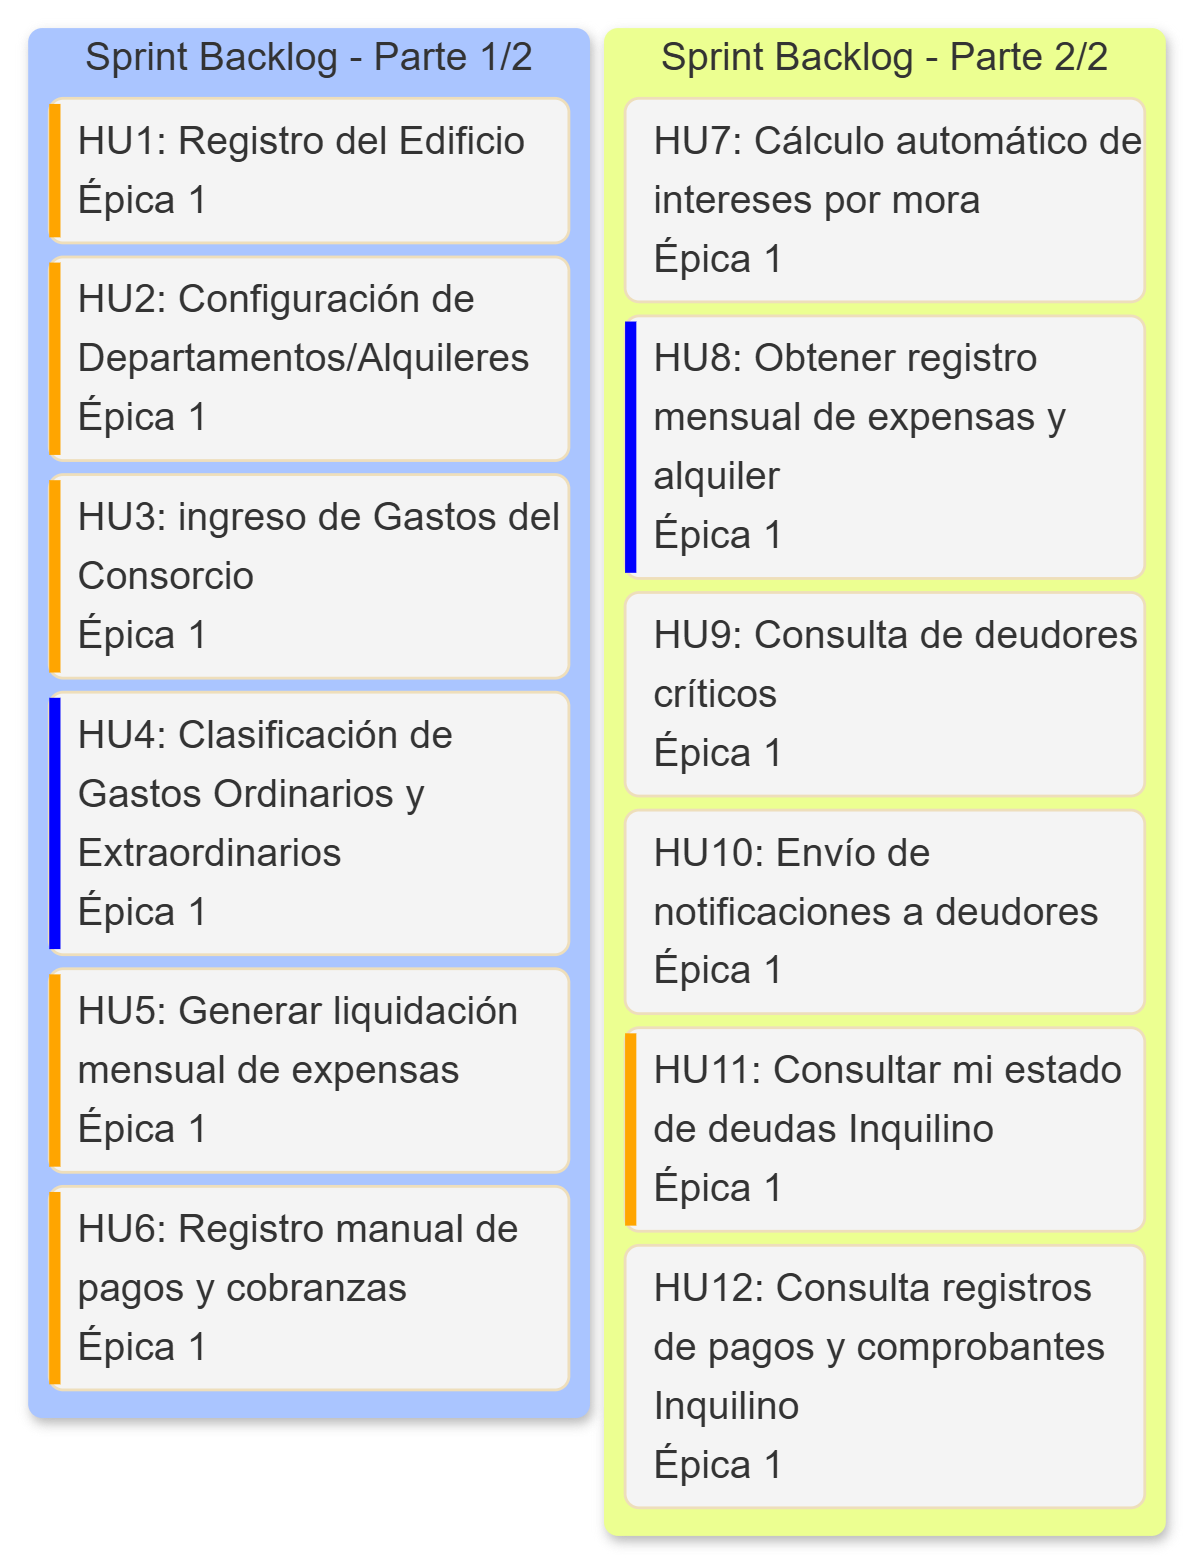
\includegraphics[width=0.7\textwidth]{figures/sprint-backlog.png}
    \caption{Mapeo de Historias de Usuario.}
\end{figure}

\paragraph{Estimación de Historias de Usuario.}
Se aplicó la técnica de \textbf{Estimación por afinidad} (Affinity Estimation), categorizando el esfuerzo y complejidad técnica del Product Backlog en tamaños relativos (Pequeño, Mediano, Grande). Esto permite al equipo alinear expectativas rápidamente, detectando que los módulos contables de prorrateo de expensas e integración de pagos representan las historias de mayor tamaño y riesgo técnico (Grande), mientras que los módulos de comunicación estimaron un esfuerzo menor (Pequeño).


\begin{figure}[H]
    \centering
    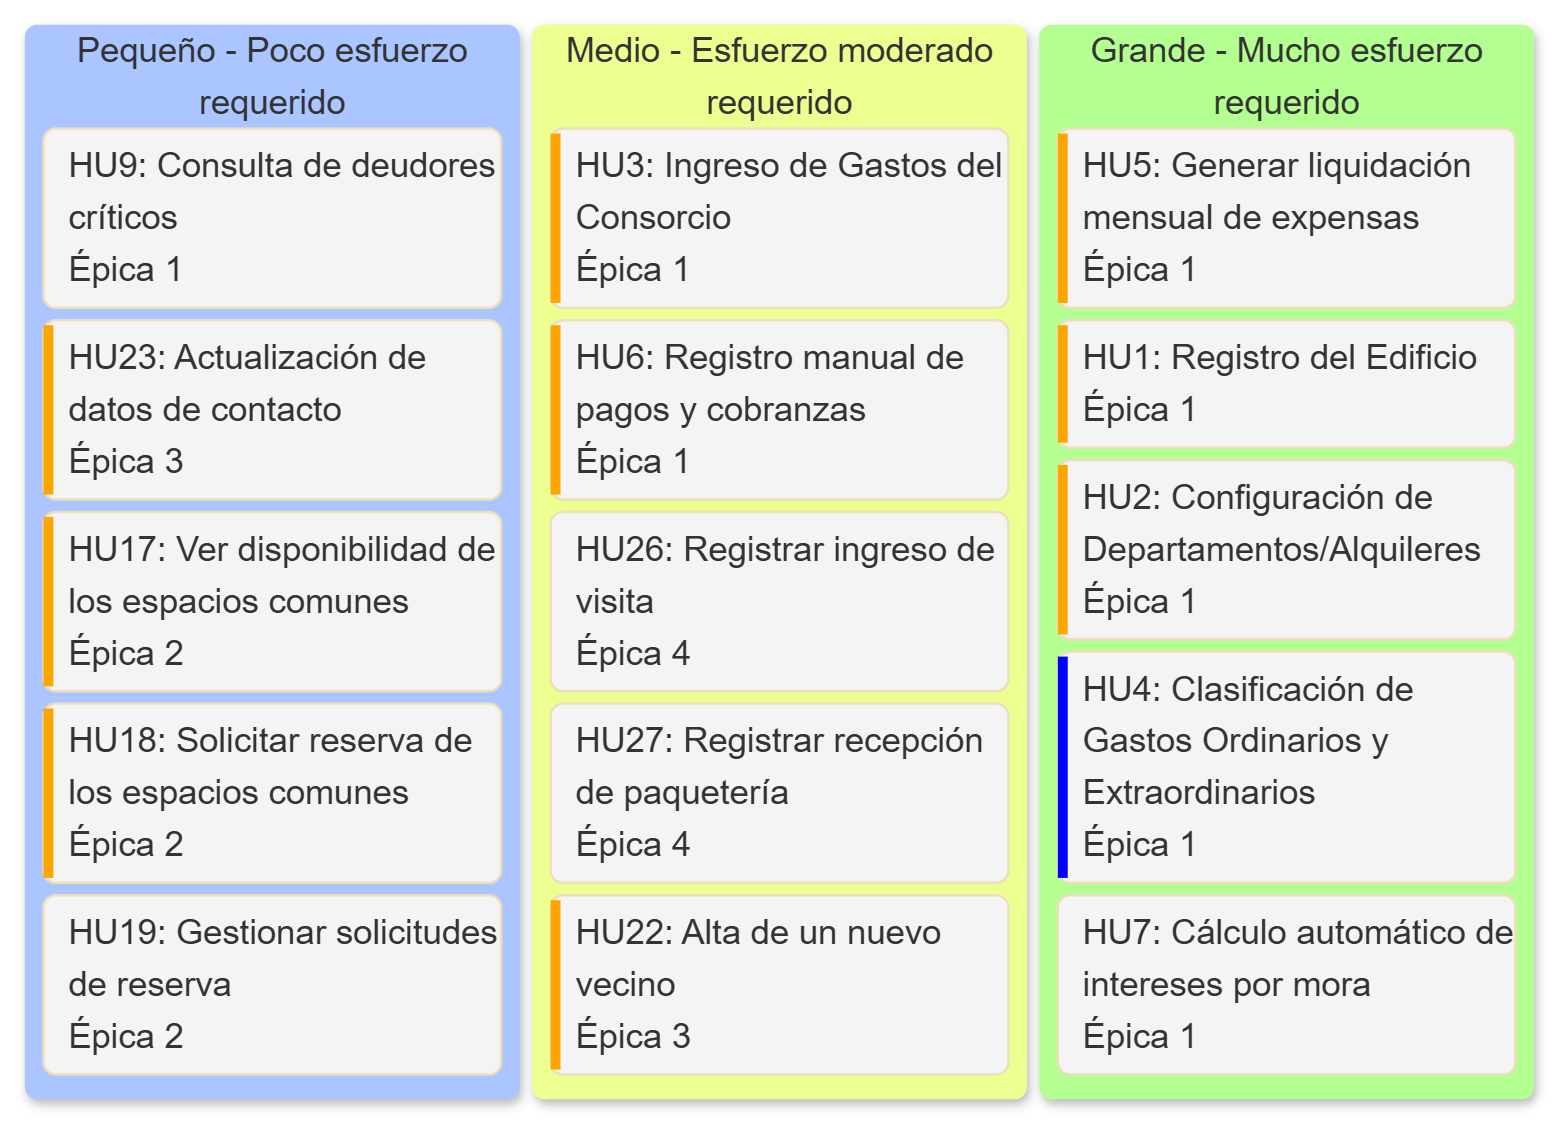
\includegraphics[width=0.8\textwidth]{figures/simulacion-de-estimacion-por-afinidad-en-trello.png}
    \caption{Simulación de Estimación por afinidad en Trello.}
\end{figure}

\paragraph{Compromiso de Historias de Usuario.}
Una vez priorizado el producto backlog y estimado el esfuerzo mediante la técnica de afinidad, el Equipo Scrum llevó a cabo la reunión de planificación del Sprint. El objetivo de la reunión fue definir el \textbf{Sprint Backlog} para el primer ciclo de desarrollo (Sprint 1), el cual cuenta con un Time-boxing de dos semanas.

Durante este proceso, el Equipo de Desarrollo evaluó su capacidad operativa y procedió a mover las historias de usuario de mayor prioridad desde la cima del Product Backlog hacia el Sprint Backlog.

Para el \textbf{Sprint 1 de la Liberación 1}, el equipo se ha comprometido formalmente a implementar las Historias de Usuario HU1 - Registro del Edificio, HU2 - Configuración de Departamentos/Alquileres, HU5 - Generar liquidación mensual de expensas, HU3 - ingreso de Gastos del Consorcio y HU6: Registro manual de pagos y cobranzas. Al tratarse de requerimientos de tamaño ``Grande'' y ``Mediano'' respectivamente, se determinó que estas historias cubren la capacidad de trabajo del equipo para esta primera iteración.

Para el \textbf{Sprint 2 de la Liberación 1}, el equipo se ha comprometido formalmente a implementar las Historias de Usuario, HU11: Consultar mi estado de deudas (Inquilino), HU15: Consultar gastos de expensa mensual (Inquilino) y HU13 - Pagar de deudas Online (Inquilino). Al tratarse de requerimientos de tamaños ``Mediano'' y ``Pequeño'', se determinó que estas historias cubren la capacidad de trabajo del equipo en esta segunda iteración.

Para el \textbf{Sprint 1 de la Liberación 2}, el equipo se ha comprometido formalmente a implementar las Historias de Usuario HU17 - Ver disponibilidad de los espacios comunes, HU18 - Solicitar reserva de los espacios comunes y HU20 - Cancelar reserva del espacio común. Se determinó que estas historias cubren la capacidad de trabajo del equipo para esta primera iteración.

Para el \textbf{Sprint 2 de la Liberación 2}, el equipo se ha comprometido formalmente a implementar Historias de Usuario HU22 - Alta de un nuevo vecino, HU23 - Actualización de datos de contacto y HU24 - Baja o desvinculación de un inquilino. Se determinó que estas historias cubren la capacidad de trabajo del equipo para esta segunda iteración.

Para el \textbf{Sprint 1 de la Liberación 3}, el equipo se ha comprometido formalmente a implementar Historias de Usuario HU26 - Registrar ingreso de visita, HU27 - Registrar recepción de paquetería y HU28 - Confirmar retiro de paquete. Se determinó que estas tareas son las que cubren la capacidad de trabajo del equipo para la primera iteración.

Para el \textbf{Sprint 2 de la Liberación 3}, el equipo se ha comprometido formalmente a implementar Historias de Usuario HU29 - Publicar un comunicado general, HU30 - Consultar documentos del consorcio y HU31 - Enviar consulta directa a la administración. Se determinó que estas tareas son las que cubren la capacidad de trabajo del equipo para la segunda iteración.

\paragraph{Identificación de Tareas.}

\begin{longtable}{|p{4.5cm}|p{10.5cm}|}
    \hline
    \textbf{Historias de Usuario} & \textbf{Tareas técnicas identificadas}
    \\ \hline
    \endhead

        \textbf{HU1 - Registro del Edificio} 
        
        & 

            \begin{enumerate}[leftmargin=*,nosep]
                \item Diseñar tabla \textit{edificios} en la base de datos.
                \item Crear Modelo y Controlador en Laravel.
                \item Desarrollar formulario de Registro (HTML/Blade).
                \item Implementar validaciones de campos (Nombre, CUIT, Dirección).
                \item Realizar pruebas de persistencia de datos.
            \end{enumerate} 
        
    \\ \hline

        \textbf{HU2: Configuración de Departamentos/Alquileres} 
        
        & 

            \begin{enumerate}[leftmargin=*,nosep]
                \item Diseñar tabla unidades \textit{vinculada} a \textit{edificios} en la base de datos.
                \item Crear lógica de asignación de coeficientes (porcentaje de las expensas).
                \item Desarrollar vista de listado de departamentos.
            \end{enumerate} 
        
    \\ \hline

        \textbf{HU3: Ingreso de Gastos del Consorcio.} 
        
        & 

            \begin{enumerate}[leftmargin=*,nosep]
                \item Diseñar tabla \textit{gastos\_consorcio}.
                \item Crear formulario de carga de facturas (Monto, Fecha, Concepto) y sección de carga de archivos.
                \item Implementar lógica de suma automática de gastos del mes.
            \end{enumerate} 
        
    \\ \hline

        \textbf{HU5 - Generar liquidación mensual de expensas} 
        
        & 

            \begin{enumerate}[leftmargin=*,nosep]
                \item Diseñar tabla \textit{liquidaciones} en la base de datos.
                \item \textbf{Crear vista (FrontEnd):} maquetar la pantalla del panel de administración que contenga el botón ``Cerrar mes'' y la ventana emergente de confirmación.
                \item \textbf{Desarrollar lógica de sumatoria (BackEnd):} programar en el controlador la consulta que sume todos los gastos cargados en el mes actual.
                \item \textbf{Desarrollar algoritmo de prorrateo:} Crear la función que tome el total de gastos y lo multiplique por el coeficiente (porcentaje) de cada unidad funcional para sacar el individual.
                \item \textbf{Generar recibos digitales:} maquetar la vista o el PDF del comprobante que verá el inquilino con su monto detallado.
                \item \textbf{Implementar validación de seguridad:} programar un bloqueo para que el administrador no pueda hacer clic en ``Cerrar mes'' dos veces para el mismo período (evitar duplicar deudas).
            \end{enumerate} 
        
    \\ \hline

        \textbf{HU6 - Registro manual de pagos y cobranzas} 
        
        & 

            \begin{enumerate}[leftmargin=*,nosep]
                \item \textbf{Diseñar} tabla \textit{pagos} en la base de datos.
                \item \textbf{Crear formulario de cobro (FrontEnd/Blade):} maquetar la pantalla para el administrador (menú desplegable de departamento y campo de monto).
                \item \textbf{Desarrollar la lógica de guardado (Backend/Controlador):} Escribir la función que guarde los datos del formulario en la tabla \textit{pagos}.
                \item \textbf{Actualizar el pago de la deuda (BackEnd):} programar lógica que busque la liquidación de ese mes y cambie el estado de ``Pendiente'' a ``Pagado''.
                \item \textbf{Generar comprobante Interno:} Maquetar una vista sencilla que muestre un resumen del pago exitoso.
            \end{enumerate} 
        
    \\ \hline

        \textbf{HU11 - Consultar mi estado de deudas (Inquilino)} 
        
        & 

            \begin{enumerate}[leftmargin=*,nosep]
                \item \textbf{Desarrollar consulta a la base de datos (BackEnd/Controlador):} buscar en la tabla de \textit{liquidaciones} el registro actual de la unidad funcional.
                \item \textbf{Crear vista principal (FrontEnd/Blade):} maquetar la pantalla ``Mis deudas'' en el panel del inquilino.
                \item \textbf{Programar lógica condicional en la Vista:} evaluar si el estado de la liquidación es ``Pendiente'' o ``Pagado''.
                \item \textbf{Maquetar escenario ``Con Deuda'' (Frontend):} diseñar la tarjeta de alerta con monto y vencimiento.
                \item \textbf{Maquetar escenario ``Sin Deuda'' (FrontEnd):} diseñar el mensaje de éxito (``Estás al día'').
            \end{enumerate} 
        
    \\ \hline

        \textbf{HU15 - Consultar gastos de expensa mensual (Inquilino)} 
        
        & 

            \begin{enumerate}[leftmargin=*,nosep]
                \item \textbf{Crear botón de acción (FrontEnd):} agregar el enlace ``ver detalle de gastos'' en la liquidación del inquilino.
                \item \textbf{Desarrollar consulta relacional (BackEnd):} buscar en la tabla \textit{gastos\_consorcio} las facturas correspondientes al mes/año.
                \item \textbf{Maquetar vista de detalle (FrontEnd):} diseñar una ventana emergente o tabla desplegable.
                \item \textbf{Formatear la salida de datos:} configurar columnas claras (Fecha, concepto, comprobante, monto) y sumatoria coincidente.
            \end{enumerate} 
        
    \\ \hline

        \textbf{HU13 - Pagar de deudas Online (Inquilino)} 
        
        & 

            \begin{enumerate}[leftmargin=*,nosep]
                \item \textbf{Investigar e integrar API de pagos:} Configurar credenciales (Tokens/Keys) en el archivo `.env`.
                \item \textbf{Crear botón de pago (Frontend/Blade):} Implementar el botón ``Pagar ahora'' capturando el monto adeudado.
                \item \textbf{Desarrollar Controlador de Integración (Backend):} Enviar datos de la deuda a la API y generar el enlace de pago seguro.
                \item \textbf{Implementar \textit{Webhook} para confirmación (Backend):} Programar ruta para recibir notificaciones de la pasarela.
                \item \textbf{Programar lógica de éxito:} Actualizar estado a ``Pagado'' al recibir estado ``Aprobado''.
                \item \textbf{Programar lógica de fallo:} Mantener estado ``Pendiente'' y mostrar error en caso de rechazo.
            \end{enumerate} 
        
    \\ \hline

        \textbf{HU18 - Solicitar reserva de los espacios comunes} 
        
        & 

            \begin{enumerate}[leftmargin=*,nosep]
                \item \textbf{Diseñar tabla en base de datos (reservas):} Crear la migración con campos requeridos.
                \item \textbf{Crear formulario de solicitud (Frontend/Blade):} Maquetar formulario con selector de fecha, invitados y reglamento.
                \item \textbf{Desarrollar lógica de validación (Backend/Controlador):} Validar fecha a futuro, checkbox y límite de invitados.
                \item \textbf{Programar lógica de guardado (Backend):} Persistir la reserva con estado inicial ``Pendiente''.
                \item \textbf{Implementar disparador de notificación (Backend):} Generar alerta interna o enviar correo al Administrador al guardar.
            \end{enumerate} 
        
    \\ \hline

        \textbf{HU20 - Cancelar reserva del espacio común} 
        
        & 

            \begin{enumerate}[leftmargin=*,nosep]
                \item \textbf{Crear interfaz de cancelación (Frontend/Blade):} Agregar botón ``Cancelar Reserva'' en reservas activas.
                \item \textbf{Desarrollar lógica de cálculo de tiempo (Backend/Controlador):} Calcular diferencia en horas respecto a la reserva.
                \item \textbf{Implementar validación condicional (Backend):} Evaluar si la diferencia es mayor a 48 horas.
                \item \textbf{Programar escenario de éxito (Criterio 1):} Actualizar estado a ``Cancelada'' y notificar al administrador.
                \item \textbf{Programar escenario de rechazo (Criterio 2):} Abortar transacción y retornar error en vista.
                \item \textbf{Maquetar alertas de retroalimentación (Frontend):} Diseñar notificaciones visuales para éxito o plazo expirado.
            \end{enumerate} 
        
    \\ \hline

        \textbf{HU17 - Ver disponibilidad de los espacios comunes} 
        
        & 

            \begin{enumerate}[leftmargin=*,nosep]
                \item \textbf{Integrar componente de calendario (Frontend):} Instalar y configurar *FullCalendar.js*.
                \item \textbf{Desarrollar consulta de rango de fechas (Backend):} Buscar reservas del mes/año actual en la base de datos.
                \item \textbf{Mapear estados de disponibilidad (Lógica de Interfaz):} Asignar clases CSS verde (disponible) o rojo (reservado/pendiente).
                \item \textbf{Programar enrutamiento:} Redirigir al clic en verde a ``Nueva Reserva'' con fecha pre-cargada.
                \item \textbf{Bloquear interacción:} Deshabilitar clics en rojo y días pasados.
            \end{enumerate} 
        
    \\ \hline

        \textbf{HU22 - Alta de un nuevo vecino} 
        
        & 

            \begin{enumerate}[leftmargin=*,nosep]
                \item \textbf{Diseñar estructura de usuarios (Base de Datos):} UNIQUE en `dni` y `email` en la tabla `users`.
                \item \textbf{Crear formulario de Alta (Frontend/Blade):} Campos de Nombre, DNI, Email y selector de unidad funcional.
                \item \textbf{Desarrollar lógica de validación (Backend/Controlador):} Validar en servidor que DNI y email sean únicos.
                \item \textbf{Programar generación de credenciales (Backend):} Generar contraseña aleatoria y encriptarla al crear el perfil.
                \item \textbf{Implementar servicio de mensajería (Backend/Mailable):} Enviar correo de bienvenida con credenciales al nuevo inquilino.
            \end{enumerate} 
        
    \\ \hline

        \textbf{HU24 - Baja o desvinculación de un inquilino} 
        
        & 

            \begin{enumerate}[leftmargin=*,nosep]
                \item \textbf{Maquetar interfaz de desvinculación (Frontend/Blade):} Botón ``Dar de baja'' y modal de confirmación.
                \item \textbf{Desarrollar lógica de Borrado Lógico (Backend):} Cambiar estado a ``Inactivo'' preservando historial.
                \item \textbf{Actualizar estado de la Unidad Funcional (Backend):} Desvincular usuario del departamento y marcarlo ``Desocupada''.
                \item \textbf{Implementar revocación de sesión activa (Seguridad):} Middleware para expulsar al usuario si está logueado.
            \end{enumerate} 
        
    \\ \hline

        \textbf{HU23 - Actualización de datos de contacto} 
        
        & 

            \begin{enumerate}[leftmargin=*,nosep]
                \item \textbf{Crear vista ``Mi Perfil'' (Frontend/Blade):} Formulario pre-cargado con información actual.
                \item \textbf{Desarrollar enrutamiento protegido (Backend):} Proteger la ruta para usuarios logueados.
                \item \textbf{Programar validación y sanitización (Backend/Controlador):} Validar formato de email y caracteres del teléfono.
                \item \textbf{Ejecutar actualización segura (Backend):} Actualizar únicamente teléfono y email del usuario logueado.
                \item \textbf{Implementar retroalimentación visual (Frontend):} Retornar a la vista con mensaje de éxito (Toast/Alert).
            \end{enumerate} 
        
    \\ \hline

        \textbf{HU26 - Registrar ingreso de visita} 
        
        & 

            \begin{enumerate}[leftmargin=*,nosep]
                \item \textbf{Diseñar tabla de auditoría (visitas):} Crear migración con campos necesarios.
                \item \textbf{Crear vista para el rol Guardia (Frontend/Blade):} Maquetar panel rápido ``Libro de Visitas''.
                \item \textbf{Desarrollar lógica de persistencia (Backend/Controlador):} Registrar datos del formulario de visitas.
                \item \textbf{Implementar sellado de tiempo automático:} Capturar hora de ingreso del servidor.
                \item \textbf{Configurar estado inicial:} Guardar con estado por defecto ``En el edificio''.
                \item \textbf{Maquetar tabla de visitas activas (Frontend):} Lista de visitas en tiempo real.
            \end{enumerate} 
        
    \\ \hline

        \textbf{HU27 - Registrar recepción de paquetería} 
        
        & 

            \begin{enumerate}[leftmargin=*,nosep]
                \item \textbf{Diseñar tabla de inventario (paquetes):} Crear migración con campos y estado ``En guardia''.
                \item \textbf{Crear formulario de recepción (Frontend/Blade):} Campos de remitente y selector de departamento.
                \item \textbf{Desarrollar Controlador de registro (Backend):} Validar e ingresar paquete asociado a la unidad.
                \item \textbf{Desarrollar lógica de notificación asíncrona (Backend):} Evento y Listener para notificar al inquilino por correo/alerta.
            \end{enumerate} 
        
    \\ \hline

        \textbf{HU28 - Confirmar retiro de paquete} 
        
        & 

            \begin{enumerate}[leftmargin=*,nosep]
                \item \textbf{Modificar vista de inventario (Frontend/Blade):} Agregar botón ``Marcar como Entregado''.
                \item \textbf{Desarrollar ruta y Controlador (Backend):} Crear método que reciba el ID del paquete.
                \item \textbf{Implementar lógica de actualización y auditoría (Backend):} Cambiar estado a ``Entregado'' y registrar hora.
                \item \textbf{Ajustar consulta de filtrado (Backend/Controlador):} Filtrar paquetes entregados de la lista de pendientes de guardia.
            \end{enumerate} 
        
    \\ \hline

        \textbf{HU29 - Publicar un comunicado general} 
        
        & 

            \begin{enumerate}[leftmargin=*,nosep]
                \item \textbf{Diseñar tabla de anuncios (comunicados):} Crear migración con campos y autor.
                \item \textbf{Crear formulario de publicación (Frontend/Blade - Admin):} Formulario para redactar avisos.
                \item \textbf{Desarrollar lógica de persistencia (Backend/Controlador):} Validar y guardar comunicado.
                \item \textbf{Implementar Colas de Trabajo (Backend):} Job para enviar correos masivos de forma asíncrona.
                \item \textbf{Modificar el Dashboard del inquilino (Frontend/Blade):} Renderizar últimos comunicados en la página de inicio.
            \end{enumerate} 
        
    \\ \hline

        \textbf{HU31: Enviar consulta directa a la administración} 
        
        & 

            \begin{enumerate}[leftmargin=*,nosep]
                \item \textbf{Diseñar tabla de mensajería (tickets o consultas):} Migración con campos e inquilino\_id.
                \item \textbf{Crear formulario de contacto (Frontend/Blade - Inquilino):} Formulario para redactar consultas.
                \item \textbf{Desarrollar lógica de persistencia (Backend/Controlador):} Guardar consulta asociada al usuario logueado.
                \item \textbf{Maquetar bandeja de entrada (Frontend/Blade - Admin):} Bandeja ordenada por fecha de creación.
                \item \textbf{Desarrollar consulta de tickets (Backend/Controlador):} Query para listar y filtrar por estado (Pendiente/Resuelto).
            \end{enumerate} 
        
    \\ \hline

        \textbf{HU30 - Consultar documentos del consorcio} 
        
        & 

            \begin{enumerate}[leftmargin=*,nosep]
                \item \textbf{Diseñar tabla de metadatos (documentos):} Crear migración con título, path y fecha.
                \item \textbf{Crear vista de repositorio (Frontend/Blade):} Grilla con íconos de los documentos del consorcio.
                \item \textbf{Desarrollar consulta de listado (Backend/Controlador):} Recuperar y enviar documentos públicos a la vista.
                \item \textbf{Implementar lógica de entrega de archivos (Backend):} Ruta de descarga segura utilizando la clase Storage.
                \item \textbf{Configurar cabeceras de respuesta HTTP:} response()-\>file() para visualización inline en el navegador.
            \end{enumerate} 
        
    \\ \hline

    \caption{Tabla de identificación de Tareas}
\end{longtable}

\paragraph{Estimación de Tareas}

\begin{longtable}{|p{10.5cm}|p{2.5cm}|c|}
    \hline
            \textbf{Historia de Usuario} 
        & 
            \textbf{Estimación de Tareas} 
        & 
            \textbf{Estimación total} 
    \\ \hline
    \endhead

            \textbf{HU1 - Registro del Edificio} 
        
        & 

            \begin{enumerate}[leftmargin=*,nosep]
                \item 2 h
                \item 1 h
                \item 2 h
                \item 3 h
                \item 2 h
            \end{enumerate} 
        
        &
        
            10 h 
        
    \\ \hline
        
            \textbf{HU2 - Configuración de Departamentos/Alquileres} 
        
        &

            \begin{enumerate}[leftmargin=*,nosep]
                \item 2 h
                \item 2 h
                \item 2 h
            \end{enumerate} 
        
        &
            8 h
    
    \\ \hline
        
            \textbf{HU3 - Ingreso de Gastos del Consorcio.} 
        
        &

            \begin{enumerate}[leftmargin=*,nosep]
                \item 2 h
                \item 1 h
                \item 2 h
            \end{enumerate} 
        
        &
            5 h
    
    \\ \hline
        
            \textbf{HU5 - Generar liquidación mensual de expensas} 
        
        &

            \begin{enumerate}[leftmargin=*,nosep]
                \item 2 h
                \item 2 h
                \item 2 h
                \item 3 h
                \item 1 h
                \item 2 h
            \end{enumerate} 
        
        &
         12 h
    \\ \hline
        
            \textbf{HU6 - Registro manual de pagos y cobranzas} 
        
        &

            \begin{enumerate}[leftmargin=*,nosep]
                \item 2 h
                \item 2 h
                \item 3 h
                \item 1 h
                \item 2 h
            \end{enumerate} 
        
        &
         10 h
    \\ \hline
        
            \textbf{HU11 - Consultar mi estado de deudas (Inquilino)} 
        
        &

            \begin{enumerate}[leftmargin=*,nosep]
                \item 2 h
                \item 2 h
                \item 1 h
                \item 3 h
                \item 2 h
            \end{enumerate} 
        
        &
            10 h
    
    \\ \hline
        
            \textbf{HU15 - Consultar gastos de expensa mensual (Inquilino)} 
        
        &

            \begin{enumerate}[leftmargin=*,nosep]
                \item 1 h
                \item 2 h
                \item 3 h
                \item 3 h
            \end{enumerate} 
        
        &
            9 h
    
    \\ \hline
        
            \textbf{HU13 - Pagar de deudas Online (Inquilino)} 
        
        &

            \begin{enumerate}[leftmargin=*,nosep]
                \item 3 h
                \item 2 h
                \item 3 h
                \item 2 h
                \item 2 h
                \item 3 h
            \end{enumerate} 
        
        &
            15 h
    
    \\ \hline
        
            \textbf{HU18 - Solicitar reserva de los espacios comunes} 
        
        &

            \begin{enumerate}[leftmargin=*,nosep]
                \item 2 h
                \item 3 h
                \item 4 h
                \item 3 h
                \item 3 h
            \end{enumerate} 
        
        &
            15 h
    
    \\ \hline
        
            \textbf{HU20 - Cancelar reserva del espacio común} 
        
        &

            \begin{enumerate}[leftmargin=*,nosep]
                \item 1 h
                \item 3 h
                \item 4 h
                \item 3 h
                \item 2 h
                \item 2 h
            \end{enumerate} 
        
        &
            15 h
    
    \\ \hline
        
            \textbf{HU17 - Ver disponibilidad de los espacios comunes} 
        
        &

            \begin{enumerate}[leftmargin=*,nosep]
                \item 2 h
                \item 3 h
                \item 3 h
                \item 4 h
                \item 3 h
            \end{enumerate} 
        
        &
            15 h
    
    \\ \hline
        
            \textbf{HU22 - Alta de un nuevo vecino} 
        
        &

            \begin{enumerate}[leftmargin=*,nosep]
                \item 2 h
                \item 2 h
                \item 3 h
                \item 4 h
                \item 5 h
            \end{enumerate} 
        
        &
            16 h
    
    \\ \hline
        
            \textbf{HU24 - Baja o desvinculación de un inquilino} 
        
        &

            \begin{enumerate}[leftmargin=*,nosep]
                \item 2 h
                \item 3 h
                \item 3 h
                \item 2 h
            \end{enumerate} 
        
        &
            10 h
    
    \\ \hline
        
            \textbf{HU23 - Actualización de datos de contacto} 
        
        &

            \begin{enumerate}[leftmargin=*,nosep]
                \item 2 h
                \item 2 h
                \item 3 h
                \item 3 h
                \item 3 h
            \end{enumerate} 
        
        &
            13 h
    
    \\ \hline
        
            \textbf{HU26 - Registrar ingreso de visita} 
        
        &

            \begin{enumerate}[leftmargin=*,nosep]
                \item 2 h
                \item 3 h
                \item 3 h
                \item 4 h
                \item 5 h
                \item 3 h
            \end{enumerate} 
        
        &
            20 h
    
    \\ \hline
        
            \textbf{HU27 - Registrar recepción de paquetería} 
        
        &

            \begin{enumerate}[leftmargin=*,nosep]
                \item 2 h
                \item 3 h
                \item 4 h
                \item 3 h
            \end{enumerate} 
        
        &
            12 h
    
    \\ \hline
        
            \textbf{HU28 - Confirmar retiro de paquete} 
        
        &

            \begin{enumerate}[leftmargin=*,nosep]
                \item 2 h
                \item 3 h
                \item 5 h
                \item 4 h
            \end{enumerate} 
        
        &
            14 h
    
    \\ \hline
        
            \textbf{HU29 - Publicar un comunicado general} 
        
        &

            \begin{enumerate}[leftmargin=*,nosep]
                \item 2 h
                \item 3 h
                \item 4 h
                \item 5 h
                \item 4 h
            \end{enumerate} 
        
        &
            18 h
    
    \\ \hline
        
            \textbf{HU31 - Enviar consulta directa a la administración} 
        
        &

            \begin{enumerate}[leftmargin=*,nosep]
                \item 3 h
                \item 3 h
                \item 3 h
                \item 2 h
                \item 2 h
            \end{enumerate} 
        
        &
            13 h
    
    \\ \hline
        
            \textbf{HU30 - Consultar documentos del consorcio} 
        
        &

            \begin{enumerate}[leftmargin=*,nosep]
                \item 2 h
                \item 3 h
                \item 4 h
                \item 3 h
                \item 2 h
            \end{enumerate} 
        
        &
            14 h
    
    \\ \hline
        
        &

        \begin{enumerate}[leftmargin=*,nosep]
          \item 2 h
          \item 3 h
          \item 4 h
          \item 3 h
          \item 2 h
        \end{enumerate} 
        
        &
         14 h \\ \hline
        
    \caption{Tabla de estimación de tareas.}
\end{longtable}

\paragraph{Actualizar el backlog del sprint}
Dado que la Liberación 1 está planificada para durar un mes en total, se dividió el trabajo en 2 Sprints de dos semanas de duración cada uno. Para el \textbf{Sprint 1}, el Backlog del Sprint se actualizó trasladando las tareas técnicas (previamente identificadas en Trello) correspondientes a las historias fundamentales (Registro de Edificio, Configuración de Unidades, Ingreso de Gastos y Liquidación Mensual). El resto de las historias de la Liberación 1 (como Consultar deudas y Pagar online) quedaron reservadas para la planificación del Sprint 2.

\subsubsection{2.1.3 - Fase - Implementación}

\paragraph{Crear entregables.}
Los desarrolladores proceden a la codificación en el framework Laravel, creando las migraciones de bases de datos, maquetando las vistas (Frontend) y programando los Controladores. A medida que las tareas avanzan, las tarjetas en el tablero Trello se mueven de la columna ``Por hacer'' a ``En progreso'' y finalmente a ``Terminada''. 

\paragraph{Realizar el Daily Standup.}
El equipo de desarrollo realiza una reunión diaria de máximo 15 minutos donde cada integrante responde tres preguntas clave: ¿Qué hice ayer para ayudar a terminar el Sprint?, ¿Qué haré hoy?, y ¿Existe algún impedimento que me bloquee? 

\paragraph{Refinar el backlog priorizado del producto.}
El Product Owner revisa las historias de usuario de futuras épicas (como el módulo del Personal de Seguridad) para asegurar que estén claras y listas para cuando inicie la planificación de las siguientes iteraciones.

\subsubsection{2.1.4 - Fase - Revisión y Retrospectiva}

\paragraph{Demostrar y validar el sprint.}
Se realiza una demostración del software funcional. Por ejemplo, el equipo muestra cómo el sistema logra tomar los gastos cargados y generar exitosamente la liquidación mensual prorrateada. Si cumple con los Criterios de Aceptación, la historia se marca como ``Hecha''. 

\paragraph{Retrospectiva del sprint.}
El equipo evalúa sus procesos internos. Se identifican aspectos positivos (ej. ``usar migraciones de Laravel agilizó el trabajo'') y áreas de mejora (ej. ``subestimamos el tiempo que tomaba maquetar las vistas'') para aplicar correcciones de cara al Sprint 2.

\subsubsection{2.1.5 - Fase - Liberación}

\paragraph{Enviar Entregables.}
El código fuente se despliega en un servidor de producción. A partir de este momento, la administración del consorcio ya cuenta con un incremento de producto funcional que pueden utilizar en su día a día para gestionar los edificios y las liquidaciones, mientras el equipo de desarrollo comienza a trabajar en la Liberación 2 (Módulo de reservas). 

\paragraph{Retrospectiva de la liberación.}
Tras completar la totalidad de las iteraciones planeadas para el cuatrimestre, se realiza una reunión global final. Se documenta la experiencia general, evaluando si el sistema cumplió con la visión original y analizando el impacto positivo de haber utilizado un marco de trabajo ágil e iterativo frente a las metodologías tradicionales.


\subsection{Entrevista}

En esta sección se detallan las entrevistas realizadas a los diferentes actores del consorcio para comprender sus necesidades y puntos de vista respecto al funcionamiento del sistema de administración.

\vspace{0.3cm}
\textbf{Entrevista 1: Administrador del Consorcio}

Se utilizó una estructura de embudo para la entrevista hacia el administrador del consorcio.  

\textbf{Preguntas abiertas:}

1. ¿Cuáles son los objetivos críticos de su departamento al administrar este edificio?

\textbf{Administrador:} ``El objetivo principal es mantener las cuentas al día para poder pagar los sueldos y los servicios sin sobresaltos. Además, necesito asegurar que el edificio esté en buenas condiciones de mantenimiento y, sobre todo, transparentar los gastos para que los vecinos no se quejen todo el tiempo. Básicamente, que la plata alcance y tener paz en el consorcio.'' 

2. Describa el proceso actual para calcular y distribuir las expensas mensuales.

\textbf{Administrador:} ``Hoy es un dolor de cabeza tremendo. A fin de mes, junto todos los tickets de gastos (luz, agua, arreglos, sueldo del encargado), los sumo en una planilla de Excel, divido por los porcentajes de cada departamento según los metros cuadrados, y armo un PDF. Después, tengo que mandarlos uno por uno por mail o imprimir los papelitos para pasarlos por debajo de la puerta. Me lleva días.''   

\textbf{Pregunta de Sondeo:} 

3. ¿Me lo puede explicar con más detalle para los casos en que hay deudores morosos? 

\textbf{Administrador:} ``Uf, ese es el mayor problema. En el Excel tengo que ir marcando quién pagó y quién no. Si alguien se atrasa, al mes siguiente tengo que acordarme de sumarle el interés punitorio del 5\% a mano sobre su deuda anterior, más la expensa nueva. A veces se me pasa, o el vecino me dice 'yo te transferí el día 15' y tengo que ir a buscar en el resumen del banco línea por línea a ver si es verdad. Es muy poco práctico.''   

\textbf{Preguntas cerradas:}

4. Mencione sus dos prioridades principales para mejorar la infraestructura de tecnología del edificio.

\textbf{Administrador:} ``Primero, automatizar el cálculo y el envío de las expensas. Segundo, tener un registro automático de los pagos para no tener que cruzar las transferencias bancarias a mano todos los días.''   

¿Cuántos subordinados tiene a cargo para el mantenimiento y seguridad que usarán el sistema?  

\textbf{Administrador:} ``Directamente relacionados con el uso del sistema, tengo a los dos guardias de seguridad que rotan en la entrada y al encargado del edificio. Tres en total.''   

\textbf{Preguntas bipolares:} 

5. ¿Desea recibir una impresión de su estado de cuenta cada mes?

\textbf{Administrador:} ``No, prefiero que quede todo 100\% digital e histórico en el sistema para poder consultarlo desde la computadora cuando quiera, sin acumular más papel.'' 

6. ¿Está de acuerdo o en desacuerdo con que el actual método manual de reservas de los espacios comunes carece de seguridad?

\textbf{Administrador:} ``Totalmente de acuerdo. Hoy con el cuaderno de papel que tiene el guardia, cualquiera tacha un nombre o se anotan dos vecinos en el mismo horario para usar los espacios comunes, y después el problema y las discusiones me explotan a mí.'' 

\vspace{0.5cm}
\textbf{Entrevista 2: Propietario/Cliente}

Para esta entrevista utilizamos la estructura de pirámide, ya que es la más acorde para el cliente.  

\textbf{Preguntas bipolares:}

1. ¿Actualmente recibe el resumen de sus expensas impreso en papel por debajo de su puerta? 

\textbf{Cliente:} ``Sí, tal cual. Me lo tiran por debajo de la puerta todos los meses.''  

\textbf{Preguntas cerradas:}

2. ¿Cuántas veces al año suele reservar los espacios comunes, como el quincho o los espacios comunes? 

\textbf{Cliente:} ``Calculale unas tres o cuatro veces al año como mucho, más que nada para algún cumpleaños o una cena familiar grande.''  

\textbf{Pregunta de Sondeo:}

3. Mencionó que el método para reservar es anotarse en un cuaderno en la guardia, ¿me puede dar un ejemplo de qué ocurre si ese cuaderno se pierde o hay doble reserva? 

\textbf{Cliente:} ``Uy, es un desastre. Una vez  organisé el cumple de mi nene, compré la comida, invité a todos, y cuando bajé al quincho con las cosas había otra familia instalada. Resulta que el guardia del turno mañana me anotó en una hoja, pero el del turno noche no lo vio y le reservó a otro vecino en el mismo horario. Nos terminamos peleando entre nosotros por culpa de la desorganización.''  

\textbf{Preguntas abiertas:}

4. ¿Cuáles son los métodos de pago electrónico que preferiría tener integrados en la nueva plataforma? 

\textbf{Cliente:} ``Para mí sería clave que tenga MercadoPago o algún QR para pagar en el momento desde el celular. Y si es transferencia bancaria, que el sistema te lo tome automático, porque hoy en día tenés que hacer la transferencia y después andar mandándole un mail al administrador con la captura de pantalla para que te lo anote. Es una pérdida de tiempo.''

5. En general, ¿qué opina de la transparencia actual en el detalle de los gastos y cómo cree que el sistema podría mejorar esa comunicación? 

\textbf{Cliente:} ``La verdad, hoy la transparencia es nula. Te llega esa hoja por debajo de la puerta con un número final gigante y un resumen que no se entiende nada. A veces dice 'Arreglo de caños: \$200.000' y vos no tenés idea de qué caño se rompió ni si pidieron presupuesto. Yo creo que si el sistema tuviera una sección tipo 'Muro' o de 'Documentos' donde suban las facturas de lo que se arregla, o un gráfico para ver en qué se nos va la plata mes a mes, nos daría muchísima más tranquilidad a todos.''

\subsection{2.3 - Especificación de requisitos de Software}

\input{sections/metodologia/2_3_ers/2_3_1_introduccion/2_3_1_1_proposito}
\input{sections/metodologia/2_3_ers/2_3_1_introduccion/2_3_1_2_alcance}
\input{sections/metodologia/2_3_ers/2_3_1_introduccion/2_3_1_3_definiciones}

\input{sections/metodologia/2_3_ers/2_3_2_descripcion/2_3_2_1_perspectiva}
\input{sections/metodologia/2_3_ers/2_3_2_descripcion/2_3_2_2_funcionalidad}
\input{sections/metodologia/2_3_ers/2_3_2_descripcion/2_3_2_3_caracteristicas_usuarios}
\input{sections/metodologia/2_3_ers/2_3_2_descripcion/2_3_2_4_restricciones}
\input{sections/metodologia/2_3_ers/2_3_2_descripcion/2_3_2_5_suposiciones_dependencias}

\subsubsection{2.3.3 - Requisitos Específicos}

Esta sección describe los requisitos funcionales y no funcionales correspondientes al Sistema de Administración de Consorcios para un Edificio.  
Los requisitos fueron definidos a partir de las funcionalidades necesarias para la gestión administrativa del consorcio y la interacción entre administradores, propietarios e inquilinos.

\paragraph{2.3.3.1 - Requisitos Funcionales}

\subparagraph{Gestión de Usuarios.}

\begin{figure}[H]
    \centering
    \begin{tabular}{|l|p{11cm}|}
    \hline
            \textbf{N° de requisito} 
        
        & 

            \textbf{Descripción del requisito} 
        
    \\ \hline
    
            \textbf{RF\#01} 
        
        & 

            El sistema debe permitir registrar usuarios ingresando sus datos personales (nombre, DNI, correo electrónico) 
        
    \\ \hline
    
            \textbf{RF\#02} 
        
        & 

            El sistema debe permitir iniciar sesión 
        
    \\ \hline
    
            \textbf{RF\#03} 
        
        & 

            El sistema debe permitir cerrar sesión 
        
    \\ \hline
    
            \textbf{RF\#04} 
        
        & 

            El sistema debe permitir actualizar datos de contacto 
        
    \\ \hline
    
            \textbf{RF\#05} 
        
        & 

            El sistema debe permitir registrar nuevos vecinos 
        
    \\ \hline
    
            \textbf{RF\#06} 
        
        & 

            El sistema debe permitir registrar bajas de inquilinos 
        
    \\ \hline
    
            \textbf{RF\#07} 
        
        & 

            El sistema debe restringir funcionalidades según el tipo de usuario 
        
    \\ \hline
    \end{tabular}
    \caption{Tabla de Requisitos: Gestión de usuarios}
\end{figure}

\subparagraph{Gestión de pagos y expensas}

\begin{figure}[H]
    \centering
    \begin{tabular}{|l|p{11cm}|}
    \hline
            \textbf{N° de requisito} 
        
        & 

            \textbf{Descripción del requisito} 
        
    \\ \hline
    
            \textbf{RF\#08} 
        
        & 

            El sistema debe permitir registrar pagos de expensas 
        
    \\ \hline
    
            \textbf{RF\#09} 
        
        & 

            El sistema debe permitir consultar historial de pagos 
        
    \\ \hline
    
            \textbf{RF\#10} 
        
        & 

            El sistema debe permitir consultar comprobantes de pago 
        
    \\ \hline
    
            \textbf{RF\#11} 
        
        & 

            El sistema debe permitir subir comprobantes de transferencia 
        
    \\ \hline
    
            \textbf{RF\#12} 
        
        & 

            El sistema debe permitir confirmar pagos realizados por transferencia 
        
    \\ \hline
    
            \textbf{RF\#13} 
        
        & 

            El sistema debe generar liquidaciones de expensas 
        
    \\ \hline
    
            \textbf{RF\#14} 
        
        & 

            El sistema debe permitir consultar estado de deuda 
        
    \\ \hline
    
            \textbf{RF\#15} 
        
        & 

            El sistema debe permitir enviar notificaciones a deudores 
        
    \\ \hline
    \end{tabular}
    \caption{Tabla de requisitos: Gestión de pagos y expensas}
\end{figure}

\subparagraph{Gestión de espacios comunes.}

\begin{figure}[H]
    \centering
    \begin{tabular}{|l|p{11cm}|}
    \hline
            \textbf{N° de requisito} 
        
        & 

            \textbf{Descripción del requisito} 
        
    \\ \hline
    
            \textbf{RF\#16} 
        
        & 

            El sistema debe permitir visualizar disponibilidad de espacios comunes 
        
    \\ \hline
    
            \textbf{RF\#17} 
        
        & 

            El sistema debe permitir solicitar reservas de espacios comunes 
        
    \\ \hline
    
            \textbf{RF\#18} 
        
        & 

            El sistema debe permitir cancelar reservas realizadas 
        
    \\ \hline
    
            \textbf{RF\#19} 
        
        & 

            El sistema debe permitir gestionar solicitudes de reserva 
        
    \\ \hline
    
            \textbf{RF\#20} 
        
        & 

            El sistema debe permitir consultar historial de reservas 
        
    \\ \hline
    \end{tabular}
    \caption{Tabla de requisitos: Gestión de espacios comunes.}
\end{figure}

\subparagraph{Gestión de visitas y paquetería.}

\begin{figure}[H]
    \centering
    \begin{tabular}{|l|p{11cm}|}
    \hline
            \textbf{N° de requisito} 
        
        & 

            \textbf{Descripción del requisito} 
        
    \\ \hline
    
            \textbf{RF\#21} 
        
        & 

            El sistema debe permitir registrar ingresos visitas 
        
    \\ \hline
    
            \textbf{RF\#22} 
        
        & 

            El sistema debe permitir registrar recepción de paquetería 
        
    \\ \hline
    
            \textbf{RF\#23} 
        
        & 

            El sistema debe permitir confirmar retiro de paquetes 
        
    \\ \hline
    \end{tabular}
    \caption{Tabla de requisitos: Gestión de visitas y paquetería.}
\end{figure}

\subparagraph{Gestión de comunicación y documentos.}

\begin{figure}[H]
    \centering
    \begin{tabular}{|l|p{11cm}|}
    \hline
            \textbf{N° de requisito} 
        
        & 

            \textbf{Descripción del requisito} 
        
    \\ \hline
    
            \textbf{RF\#24} 
        
        & 

            El sistema debe permitir publicar comunicados generales 
        
    \\ \hline
    
            \textbf{RF\#25} 
        
        & 

            El sistema debe permitir consultar documentos del consorcio 
        
    \\ \hline
    
            \textbf{RF\#26} 
        
        & 

            El sistema debe permitir enviar consultas directas a la administración 
        
    \\ \hline
    \end{tabular}
    \caption{Tabla de requisitos: Gestión de comunicación y documentos.}
\end{figure}

\subparagraph{Gestión de departamentos y contratos}

\begin{figure}[H]
    \centering
    \begin{tabular}{|l|p{11cm}|}
    \hline
            \textbf{N° de requisito} 
        
        & 

            \textbf{Descripción del requisito} 
        
    \\ \hline
    
            \textbf{RF\#27} 
        
        & 

            El sistema debe permitir registrar departamentos 
        
    \\ \hline
    
            \textbf{RF\#28} 
        
        & 

            El sistema debe permitir asociar propietarios a departamentos 
        
    \\ \hline
    
            \textbf{RF\#29} 
        
        & 

            El sistema debe permitir registrar contratos de alquiler 
        
    \\ \hline
    
            \textbf{RF\#30} 
        
        & 

            El sistema debe permitir consultar contratos activos 
        
    \\ \hline
    
            \textbf{RF\#31} 
        
        & 

            El sistema debe permitir la integración con pasarelos de pagos externos. 
        
    \\ \hline
    \end{tabular}
    \caption{Tabla de requisitos: Gestión de comunicación y contratos.}
\end{figure}

\input{sections/metodologia/2_3_ers/2_3_4_no_funcionales/2_3_4_1_producto}
\input{sections/metodologia/2_3_ers/2_3_4_no_funcionales/2_3_4_2_organizacionales}
\input{sections/metodologia/2_3_ers/2_3_4_no_funcionales/2_3_4_3_externos}


\subsection{2.4 - Análisis de Riesgos}

La gestión de riesgos constituye un proceso fundamental para asegurar el éxito del presente proyecto, permitiendo la identificación, análisis y mitigación proactiva de los factores que podrían comprometer sus objetivos. Dada la naturaleza dinámica de nuestro ``Sistema de Administración de Consorcios'', el enfoque adoptado se basa en un marco de trabajo continuo que abarca cuatro etapas críticas: la identificación de amenazas potenciales para el negocio, el producto y el cronograma del proyecto; el análisis cualitativo de su probabilidad e impacto; la planificación de estrategias de prevención y contingencia; y, finalmente, la supervisión constante para ajustar las medidas de control según la evolución del desarrollo.  

Este análisis permite al equipo anticipar posibles dificultades, optimizar la asignación de recursos y garantizar la calidad y fiabilidad del software final frente a incertidumbres tanto técnicas como organizacionales.

\begin{figure}[H]
    \centering
    \begin{tabularx}{\textwidth}{|p{5cm}|p{3cm}|X|}
    \hline
            \textbf{Riesgo} 
        
        & 
        
            \textbf{Tipo} 
        
        & 
        
            \textbf{Descripción} 
        
    \\ \hline
    
            \textbf{Error en cálculos financieros} 
        
        & 
        
            Producto 
        
        & 
        
            Errores en la lógica del prorrateo automático de expensas o en el cálculo de intereses por mora. 
        
    \\ \hline
    
            \textbf{Falla en seguridad de datos} 
        
        & 
        
            Producto 
        
        & 
        
            Acceso no autorizado o filtración de datos sensibles de los vecinos y registros del Libro de Visitas. 
        
    \\ \hline
    
                \textbf{Falla de integración de pagos} 
        
        & 
        
            Proyecto (producto) 
        
        & 
        
            Problemas técnicos al conectar el sistema con la pasarela de pagos para la generación de recibos. 
        
    \\ \hline
    
            \textbf{Nuevos requerimientos del cliente} 
        
        & 
        
            Negocio 
        
        & 
        
            Solicitud de cambios o nuevas funciones (ej. agregar un módulo de votación a mitad del desarrollo). 
        
    \\ \hline
    
            \textbf{Baja adopción tecnológica} 
        
        & 
        
            Negocio 
        
        & 
        
            Resistencia de los vecinos (especialmente adultos mayores) a utilizar la aplicación para reservas o pagos. 
        
    \\ \hline
    
            \textbf{Falta de experiencia técnica} 
        
        & 
        
            Proyecto 
        
        & 
        
            Dificultad para manejar las herramientas de desarrollo elegidas para el módulo de notificaciones push. 
        
    \\ \hline
    
            \textbf{Interfaz poco intuitiva} 
        
        & 
        
            Producto 
        
        & 
        
            Diseño de pantallas confuso que dificulte la carga de tickets de mantenimiento por parte del vecino. 
        
    \\ \hline
    
            \textbf{Ausencia de integrantes} 
        
        & 
        
            Proyecto 
        
        & 
        
            Inasistencia de un miembro del equipo por razones de salud o personales durante las fechas de entrega. 
        
    \\ \hline
    \end{tabularx}
    \caption{Tabla de los riesgos que se pensaron}
\end{figure}

Tras la identificación, se procede a la valoración cualitativa de cada riesgo (Probabilidad y Seriedad). Finalmente, se define el plan de gestión y la estrategia de mitigación para cada uno.

\begin{figure}[H]
    \centering
    \begin{tabularx}{\textwidth}{|X|l|l|}
    \hline
            \textbf{Riesgo} 
        
        & 
        
            \textbf{Probabilidad} 
        
        & 
        
            \textbf{Seriedad} 
        
    \\ \hline
    
            \textbf{Falla de seguridad de datos} 
        
        & 
        
            Baja 
        
        & 
        
            Alta 
        
    \\ \hline
    
            \textbf{Error en cálculos financieros} 
        
        & 
        
            Media 
        
        & 
        
            Alta 
        
    \\ \hline
    
            \textbf{Ausencia de integrantes} 
        
        & 
        
            Media 
        
        & 
        
            Alta 
        
    \\ \hline
    
            \textbf{Nuevos requerimientos del cliente} 
        
        & 
        
            Alta 
        
        & 
        
            Media 
        
    \\ \hline
    
            \textbf{Baja adopción tecnológica} 
        
        & 
        
            Media 
        
        & 
        
            Media 
        
    \\ \hline
    
            \textbf{Falla de integración de pagos} 
        
        & 
        
            Alta 
        
        & 
        
            Media 
        
    \\ \hline
    
            \textbf{Falta de experiencia técnica} 
        
        & 
        
            Media 
        
        & 
        
            Baja 
        
    \\ \hline
    
            \textbf{Interfaz poco intuitiva} 
        
        & 
        
            Baja 
        
        & 
        
            Baja 
        
    \\ \hline
    \end{tabularx}
    \caption{Tabla con las probabilidades y seriedad de los riesgos}
\end{figure}

A continuación, se detalla la estrategia de gestión y el plan de acción específico para la prevención o mitigación de cada riesgo.

\begin{figure}[H]
    \centering
    \begin{tabularx}{\textwidth}{|p{5.5cm}|p{2.5cm}|X|}
    \hline
        \textbf{Riesgo} 
        
        & 
        
            \textbf{Estrategia} 
        
        & 
        
            \textbf{Plan de Gestión (Detalle)} 
        
    \\ \hline
    
            \textbf{Falla de seguridad de datos} 
        
        & 
        
            Prevención 
        
        & 
        
            Implementar cifrado de datos sensibles y auditorías de acceso desde la fase de diseño. 
        
    \\ \hline
    
            \textbf{Error en cálculos financieros} 
        
        & 
        
            Prevención 
        
        & 
        
            Realizar pruebas unitarias intensivas sobre la lógica del prorrateo y validaciones cruzadas. 
        
    \\ \hline
    
            \textbf{Ausencia de integrantes} 
        
        & 
        
            Minimización 
        
        & 
        
            Documentar todo el código y procesos para que cualquier miembro pueda retomar tareas de otro. 
        
    \\ \hline
    
            \textbf{Nuevos requerimientos del cliente} 
        
        & 
        
            Prevención 
        
        & 
        
            Establecer un alcance claro (Scope) y utilizar un mecanismo formal de gestión de cambios. 
        
    \\ \hline
    
            \textbf{Baja adopción tecnológica} 
        
        & 
        
            Minimización 
        
        & 
        
            Crear tutoriales breves y realizar una prueba de usabilidad con un grupo control de adultos mayores. 
        
    \\ \hline
    
            \textbf{Falla de integración de pagos} 
        
        & 
        
            Contingencia 
        
        & 
        
            Tener un plan de respaldo manual para la generación de recibos si la API de pago falla. 
        
    \\ \hline
    
            \textbf{Falta de experiencia técnica} 
        
        & 
        
            Prevención 
        
        & 
        
            Capacitación temprana mediante workshops técnicos o tutoriales sobre notificaciones push. 
        
    \\ \hline
    
            \textbf{Interfaz poco intuitiva} 
        
        & 
        
            Prevención 
        
        & 
        
            Realizar prototipado rápido y validación con usuarios reales antes de la codificación final. 
        
    \\ \hline
    \end{tabularx}
    \caption{Estrategias para cada riesgo}
\end{figure}

\subsubsection{2.5 - Planificación del Proyecto}

La planificación del Sistema de Administración de Consorcio se rige bajo la metodología ágil Scrum, estructurando el trabajo mediante iteraciones denominadas Sprints. Se ha definido un esquema de entregas basado en el valor de negocio, segmentado en tres grandes liberaciones con un Time-boxing de dos semanas por cada Sprint.

\paragraph{2.5.1 - Liberación 1: Gestión Financiera Base}
Esta liberación constituye el núcleo empírico del sistema.
\begin{itemize}
    \item \textbf{Sprint 1:} Comprende la configuración estructural y el motor contable.  
    \textbf{Historias comprometidas:} HU1 (Registro del Edificio), HU2 (Configuración de Departamentos), HU3 (Ingreso de Gastos), HU5 (Generar liquidación), y HU6 (Registro manual de pagos).  
    \textbf{Esfuerzo total estimado:} 45 h
    
    \item \textbf{Sprint 2:} Enfocado en la visibilidad y métodos de pago para el usuario final.  
    \textbf{Historias comprometidas:} HU11 (Consultar deudas), HU15 (Consultar gastos), y HU13 (Pagar deudas Online).  
    \textbf{Esfuerzo total estimado:} 34 h
\end{itemize}

\paragraph{2.5.2 - Liberación 2: Gestión de Espacios y Usuarios}

Expande el valor entregado incorporando la operatividad diaria del residente.
\begin{itemize}
    \item \textbf{Sprint 1:} Centrado en el módulo de reservas.  
    \textbf{Historias comprometidas:} HU17 (Ver disponibilidad), HU18 (Solicitar reserva), y HU20 (Cancelar reserva).  
    \textbf{Esfuerzo total estimado:} 45 h
    
    \item \textbf{Sprint 2:} Dedicado a la gestión del padrón de vecinos.  
    \textbf{Historias comprometidas:} HU22 (Alta de vecino), HU23 (Actualización de datos), y HU24 (Baja/desvinculación).  
    \textbf{Esfuerzo total estimado:} 39 h
\end{itemize}

\paragraph{2.5.3 - Liberación 3: Seguridad y Transparencia}

Abarca las funcionalidades operativas para el control físico y la comunicación institucional.
\begin{itemize}
    \item \textbf{Sprint 1:} Implementación del libro digital de guardia.  
    \textbf{Historias comprometidas:} HU26 (Ingreso de visita), HU27 (Recepción de paquetería), y HU28 (Confirmar retiro).  
    \textbf{Esfuerzo total estimado:} 46 h
    
    \item \textbf{Sprint 2:} Módulo de comunicación y repositorio documental.  
    \textbf{Historias comprometidas:} HU29 (Publicar comunicado), HU30 (Consultar documentos), y HU31 (Enviar consulta).  
    \textbf{Esfuerzo total estimado:} 45 h
\end{itemize}

\paragraph{2.5.4 - Actividades y Ceremonias Ágiles}

Durante el desarrollo de estos Sprints, el equipo ejecutará las siguientes ceremonias:
\begin{itemize}
    \item \textbf{Daily Standup:} Reuniones diarias para sincronizar tareas respondiendo qué se hizo, qué se hará y qué impedimentos existen.  
    \item \textbf{Revisión del Sprint:} Demostración del software funcional al finalizar la iteración para validar los criterios de aceptación.  
    \item \textbf{Retrospectiva del Sprint:} Evaluación de procesos internos para identificar áreas de mejora y optimizar el flujo de trabajo en la siguiente iteración.
\end{itemize}



%--------------------------------------------------
\newpage

%------------------ Herramientas ------------------
\section{Herramientas y/o lenguajes de programación}

Dado que la presente etapa del proyecto ``CoConsorcio'' se centró en el relevamiento, la especificación de requisitos y la simulación de la gestión bajo un marco de trabajo ágil, no se emplearon lenguajes de programación ni entornos de desarrollo de código. En su lugar, el equipo hizo uso exclusivo de herramientas de software orientadas a la administración de proyectos, la redacción colaborativa y la comunicación.  

A continuación, se describen brevemente las herramientas utilizadas:

\begin{itemize}
    \item \textbf{Google Docs:} Procesador de textos basado en la nube utilizado para la redacción colaborativa en tiempo real. Fue la herramienta principal para estructurar, revisar y unificar toda la documentación académica del proyecto, incluyendo la Especificación de Requisitos de Software (ERS) y la transcripción de entrevistas.  
    \item \textbf{Trello:} Software de administración de proyectos basado en la metodología de tableros visuales Kanban. Se utilizó para simular y gestionar el ciclo de vida del marco de trabajo Scrum, permitiendo al equipo administrar el \textit{Product Backlog}, planificar los Sprints y realizar el seguimiento del estado de las Historias de Usuario.  
    \item \textbf{Gemini (Inteligencia Artificial):} Asistente basado en modelos de lenguaje de gran tamaño (LLM) empleado como herramienta de apoyo metodológico. Se utilizó para estructurar ideas, refinar la redacción técnica de los requerimientos bajo el estándar IEEE y generar escenarios de simulación (datos de prueba para entrevistas e historias de usuario).  
    \item \textbf{Discord:} Plataforma de comunicación mediante canales de voz y texto. Se empleó para llevar a cabo las reuniones sincrónicas del equipo, especialmente para coordinar las tareas, simular las reuniones ágiles (\textit{Daily Standups}) y compartir pantalla durante la revisión de los documentos.  
    \item \textbf{WhatsApp:} Aplicación de mensajería instantánea utilizada como canal secundario para la comunicación asincrónica y rápida del equipo. Facilitó la organización de horarios, avisos urgentes y el intercambio de enlaces directos a los recursos del proyecto.  
\end{itemize}

%--------------------------------------------------

\end{document}